\chapter[Motor Control I: The Brain as Controller]{Motor Control I:\\The Brain as Controller}
\label{ch:motor_control_brain}
\index{spinal cord}
\index{sampling rate}
\index{recruitment order}
\index{predictive processing}
\index{prediction error}
\index{optimal control}
\index{open-loop control}
\index{nonlinear control}
\index{neural computation}
\index{muscle unit recruitment}
\index{motor units}
\index{motor planning}
\index{motor cortex}
\index{inverse model}
\index{internal models}
\index{ideomotor theory}
\index{free energy principle}
\index{forward model}
\index{feedforward control}
\index{feedback control}
\index{dopamine}
\index{control bandwidth}
\index{computational capacity}
\index{closed-loop control}
\index{cerebellum}
\index{cerebellar learning}
\index{brain power consumption}
\index{basal ganglia}
\index{bandwidth limitation}
\index{active inference}
\index{action selection}
\index{action effect}
\index{Purkinje cells}
\index{Henneman's size principle}
\raggedbottom

\begin{laymansbox}{What This Chapter Is About}{box:ch24_intro}
A golf swing joins a physical system to a nervous system that prepares, senses, predicts and learns. Muscles supply and absorb energy; the body's geometry and connections distribute force and motion. A useful controller must work with both. The scientific question is how preparation and ongoing regulation combine to achieve a strike despite uncertainty and limited time.

Engineering models make this question precise. They do not establish that a particular brain region literally solves our equations. We will distinguish a mechanical identity, a proposed control architecture and an experimental finding. The strongest argument for exploiting mechanical structure comes from showing what it changes in the task, not from declaring the swing passive or the brain too slow to participate.
\end{laymansbox}

\section{The Control Problem: What the Brain Must Solve}
\label{sec:ch24_control_problem}
\label{constr:box:ch24_constraints}
For an unconstrained rigid model in local generalized coordinates, let $q\in\mathbb R^n$ and $v=\dot q$. With generalized torque $u\in\mathbb R^m$ applied through $B(q)$,
\begin{equation}
\dot x=f(x)+G(x)u,\qquad
x=\begin{bmatrix}q\\v\end{bmatrix},\quad
f=\begin{bmatrix}v\\-M^{-1}(c+g)\end{bmatrix},\quad
G=\begin{bmatrix}0\\M^{-1}B\end{bmatrix}.
\label{eq:ch24_control_affine}
\end{equation}
Here $M$ is the positive-definite mass matrix, $c$ is the complete velocity-dependent bias and $g$ is gravitational loading. Drift includes the kinematic block $v$; it is not a source of free energy or a substitute for muscle work. Contact constraints change the equations and admissible motions. A moving base, both arms, flexible tissues and a flexible club require their corresponding states and force laws.

The input in this equation is generalized torque, not a cortical spike or a muscle excitation. A more physiological model might use neural drive $e$, activation $a$, muscle-tendon state $z$ and muscle forces $F_m$:
\[
\dot a=\mathcal A(a,e),\qquad \dot z=\mathcal Z(z,q,v,a),\qquad
\tau_m=R(q)F_m(q,v,a,z).
\]
The moment-arm matrix $R$ maps muscle forces to joint torques. This map is generally redundant, state dependent and subject to unilateral force and activation bounds. Two activation patterns can produce the same net torque but different stiffness, metabolic cost and future force capacity. Adding activation and material memory to the state changes the control problem; a torque-level affine representation does not automatically remain affine in every proposed neural input.

The task is also more specific than reproducing a joint trajectory. Club position, velocity, face orientation and contact conditions jointly influence a strike; ball flight and ground interaction then introduce further states and uncertainty. A state estimate, an admissible input set and a defined task loss are needed before an optimal-control comparison is meaningful.

\begin{definition}{Feedback and Feedforward in One Policy}{ch24_feedback}
Feedback makes a command depend on available observations or an estimate derived from them. A local engineering example is
\[
u(t)=\operatorname{proj}_{\mathcal U}
\left[u_{\rm ff}(t)+K(t)\bigl(x_d(t)-\hat x(t)\bigr)\right].
\]
The projection denotes the nearest admissible torque under a declared metric and a closed convex set $\mathcal U$; more complicated actuator constraints require their own allocation rule. $K$ maps state error into torque with compatible units. Neither this proportional law nor its stability is a universal property of neural control.
\end{definition}
\begin{definition}{Prepared Commands and Feedback Policies}{ch24_feedforward}
A feedforward component is prepared without depending on the corresponding newly arriving sensory consequence. It can be learned without explicitly identifying a physical model. A prepared command and a prepared feedback policy can operate together: learning the latter does not make execution open-loop.
\end{definition}
\label{subsec:ch24_ff_vs_fb}
\label{myth:box:ch24_feedback_fantasy}

The sensory system observes outputs rather than an exact instantaneous state. A schematic channel $\ell$ gives
\[
y_\ell(t)=h_\ell\bigl(x(t-d_\ell)\bigr)+\nu_\ell(t),
\]
where $d_\ell$ is its defined delay and $\nu_\ell$ is measurement error. A delayed observation must be compared with a prediction for the same time and sensory quantity. An estimator may correct its past estimate and propagate the correction forward using intervening commands. It cannot remove uncertainty merely by predicting, and it cannot infer unobservable states uniquely from insufficient measurements.

\begin{example}{Delays in the Golf Swing}{ch24_delay_golf}
Short-latency upper-limb stretch responses are often discussed in approximate onset bands of 20--45 ms, long-latency responses in 50--100 ms, and voluntary responses at greater than 100 ms. These are exemplar EMG-response bands from specific experiments, not universal golf constants or complete times to change club motion \citep{kurtzer2014longlatency,pruszynski2012longlatency}. Parallel pathways do not form a single serial sum.

Neural conduction, sensory processing, activation and force transmission must be defined separately. If a measured latency already ends at force onset, adding a second full electromechanical delay would double-count processes. Late visually guided corrections may have little time to affect impact, while earlier task-dependent feedback may influence muscle activity, impedance or trajectory. Response authority means the attainable change in a specified mechanical outcome, not simply whether an EMG response has begun.
\end{example}

\section{Internal Models: Prediction, Inversion and Feasibility}
\label{sec:ch24_internal_models}
An internal forward model is a functional hypothesis about prediction. Evidence for prediction does not imply a conscious simulation, an exact neural copy of rigid-body mechanics or one unique implementation. In a human hand-localization experiment with movements in darkness and externally imposed forces, Wolpert and colleagues tested state estimation that combines sensory information with motor-command information \citep{Wolpert1995Integration}. That task supports a predictive-estimation account; it does not identify a golf-swing control law.

\begin{definition}{A Dimensionally Consistent Forward Model}{ch24_forward_model}
If $\hat f$ and $\hat G$ predict a continuous-time state derivative, a first-order discrete prediction is
\[
\hat x_{k+1}^{-}=\hat x_k^{+}
+\Delta t\left[\hat f(\hat x_k^{+})+\hat G(\hat x_k^{+})u_k\right].
\]
The superscripts distinguish before and after measurement correction. A derivative must be multiplied by time and added to a state. Alternatively define a discrete transition $\hat x_{k+1}^{-}=F_{\Delta t}(\hat x_k^{+},u_k)$; it is a different object from the vector field. For a smooth model, one Euler step has local error of order $\Delta t^2$, while accumulated error over a fixed interval is generally first order.
\end{definition}

A sensory prediction is $\hat y_k=h(\hat x_k^-)$, not necessarily $\hat x_k^-$. For a linear measurement, an illustrative estimator update is $\hat x_k^+=\hat x_k^-+L_k(y_k-H\hat x_k^-)$. The innovation is a sensory discrepancy. Its gain depends on modeled uncertainty, observability and the estimation objective; it is not obtained by treating every sensory channel as equally reliable. In nonlinear, constrained or delayed systems this simple update needs appropriate extensions.

\begin{definition}{Inverse Control With a Feasibility Residual}{ch24_inverse_model}
For a desired derivative, define $b=\dot x_d-\hat f(\hat x)$. The matrix $\hat G$ is $2n\times m$ in the torque model and has a zero position block. It generally has no ordinary inverse. Exact instantaneous realization requires $b\in\hat G\mathcal U$. A bounded allocation can instead solve
\[
u^\star=\arg\min_{u\in\mathcal U}
\left[\tfrac12\lVert\hat G u-b\rVert_W^2+
\tfrac\lambda2\lVert u\rVert_V^2\right],\qquad
r=b-\hat G u^\star.
\]
$W$ and $V$ specify units, scaling and priorities; $\lambda\geq0$ sets regularization. The feasibility residual $r$ must be reported. A pseudoinverse alone supplies neither actuator feasibility nor an exact solution outside the range. When an exact solution exists without bounds, null-space inputs may remain undetermined.
\end{definition}

For full joint actuation, inverse dynamics can instead compute $u=M\ddot q_d+c+g$ along a kinematically consistent desired trajectory. This still requires torque feasibility and a controller for deviations. It does not identify individual muscles. Differentiating a forward model yields sensitivities; turning those into a useful inverse requires a well-posed constrained problem, not merely writing an inverse symbol.

\begin{example}{A Rectangular Input Cannot Set Every Derivative}{ch24_no_model}
Use explicitly normalized state and input coordinates, $f=(v_1,v_2,0,0)^T$, and $G=(0,0,1,1)^T$. Suppose $b=(0,1,3,0)^T$. No input can realize the requested extra position derivative, and one shared input cannot simultaneously produce accelerations 3 and 0. With identity weighting the unconstrained least-squares input is 1.5; with $|u|\leq1$ it is 1, leaving $r=(0,1,2,-1)^T$. This residual is a physical limitation of the declared map, not a numerical solver failure.

Instantaneous rank deficiency does not by itself prove finite-time uncontrollability. The double-integrator position block is zero, yet acceleration changes later position. That distinction is essential when connecting drift, instantaneous ratios and reachable strike outcomes.
\end{example}
\label{subsec:ch24_why_models_matter}

\subsection{The Cerebellum and the Limits of a Neural Interpretation}
\label{subsec:ch24_cerebellum}
\label{princ:box:ch24_cerebellum_arch}
The cerebellum contributes to coordination and adaptation, but ``the body's simulator'' is a functional metaphor, not a complete anatomical explanation. A lesion does not selectively delete a line of pseudocode. Symptoms and retained skills vary; a diagnosis cannot establish that every affected person is unable to strike a ball or make a smooth reach.

A widely studied hypothesis links climbing-fiber activity, Purkinje-cell activity and plasticity at parallel-fiber synapses. It is not a universal scalar gradient-descent algorithm. In experiments on three genetically altered mouse lines lacking the tested form of cerebellar long-term depression, Schonewille and colleagues found preserved learning in their tested paradigms; they also explicitly considered alternative and compensatory mechanisms \citep{schonewille2011ltd}. This limits a claim that that one plasticity mechanism is necessary for all cerebellar learning. It does not show that the cerebellum or LTD is irrelevant to learning.

\begin{example}{A Learning Rule Requires a Defined Objective}{box:ch24_cerebellum_arch}
For a declared linear predictor $\hat y=w^T\phi$ and target $y$, set $e=\hat y-y$ and $\mathcal L=\tfrac12 e^2$. Gradient descent gives
\begin{equation}
\Delta w=-\eta e\phi.
\label{eq:ch24_cerebellar_learning}
\end{equation}
This is a mathematical derivation for that predictor. If the output nonlinearity or loss changes, so does the gradient. An additional postsynaptic-rate factor requires a justified model. A signed error can yield positive or negative updates; a minus sign alone does not establish synaptic depression, stable learning or a biological implementation. Temporal credit assignment additionally requires specifying which past activity is eligible for modification.
\end{example}

\section{Predictive Processing and Distinct Kinds of Error}
\label{sec:ch24_predictive_processing}
Prediction enters several theories of motor control. Predictive processing, active inference and optimal feedback control are related research programs with different assumptions; success on one prediction task does not establish them as interchangeable or settled descriptions of the whole brain. A forward model can appear inside a feedback controller without committing to a free-energy account.

\begin{definition}{Prediction, Task and Reward Errors}{ch24_predictive_processing}
A sensory prediction error compares an observation with its predicted sensory consequence. A task error compares an achieved outcome with a desired outcome. A reward prediction error compares received and expected value. These quantities can disagree. A golfer may correctly predict a miss, producing little sensory surprise but a large target error. A successful shot may still be unexpectedly good or entirely expected.
\end{definition}

For a normalized belief distribution $q(z)$ over latent states and a generative joint probability $p(y,z)$, variational free energy is
\[
\mathcal F[q]=\mathbb E_q[\log q(z)-\log p(y,z)]
=D_{\rm KL}\bigl(q(z)\Vert p(z\mid y)\bigr)-\log p(y).
\]
This identity requires suitable support and finite expectations. Its nonnegative KL term makes it an upper bound on negative log evidence. It is an information quantity, not tissue energy measured in joules. Active-inference models must additionally specify actions, beliefs, preferred outcomes and their optimization; simply imagining a target is not a mathematical definition of active inference \citep{Friston2010ActionModel}.

The identity does not prove that biological neurons minimize this objective. Nor does low prediction error imply a good golf shot: an accurately predicted error remains an error relative to the task. A useful scientific comparison asks competing models to predict different responses to sensory changes, rewards or mechanical perturbations, then tests those responses.

\section{Ideomotor Theory and Task-Oriented Instruction}
\label{sec:ch24_ideomotor}
\label{thm:ch24_ideomotor}
Ideomotor accounts propose that learned links between actions and their sensory effects contribute to action selection \citep{hommel2009theory}. This motivates a hypothesis about recalling an action through a desired effect. It is not a theorem that all movement is represented only as effects, that mechanical instruction confuses a motor system, or that thinking about a target selects a uniquely correct muscle sequence.

\begin{principle}{Effects Do Not Determine One Motor Solution}{ch24_ideomotor}
Several body motions may produce similar ball flights, while similar felt motions may produce different strikes. Selecting an effect leaves questions about state estimation, feasible actuation, robustness and credit assignment. An outcome goal and mechanical knowledge can inform the same learning process.
\end{principle}

In an engineering formulation, a task objective can penalize strike error and effort without requiring every joint to follow a prescribed path. Stochastic optimal feedback control provides one formal account of allowing variation in directions that do not interfere with the goal \citep{Todorov2002}. That prediction depends on the cost, dynamics and uncertainty model. It does not imply that any joint can be ignored throughout a swing or that all variation is beneficial.

A coaching comparison therefore needs more than two attractive slogans. Specify the cue, skill level, task and outcome; compare retention and transfer as well as immediate performance. A cue about club motion may be an external effect even though it contains mechanics. A cue about bodily feeling may direct attention internally even though it contains no joint terminology. Ideomotor theory alone cannot rank these instructions or prescribe one for every golfer. The chapter's role is to identify testable alternatives.

\section{Distributed Neural Contributions and the Mechanical System}
\label{sec:ch24_architecture}
\label{sec:ch24_hardware}
The nervous system contains interacting cortical, subcortical, brainstem, cerebellar and spinal circuits. A serial diagram from ``goal center'' to ``muscles'' omits recurrent communication and sensory dependence. The figure separates functional roles without assigning each role to a single neural structure or inventing one clock rate for each box.

\begin{figure}[p]
\centering
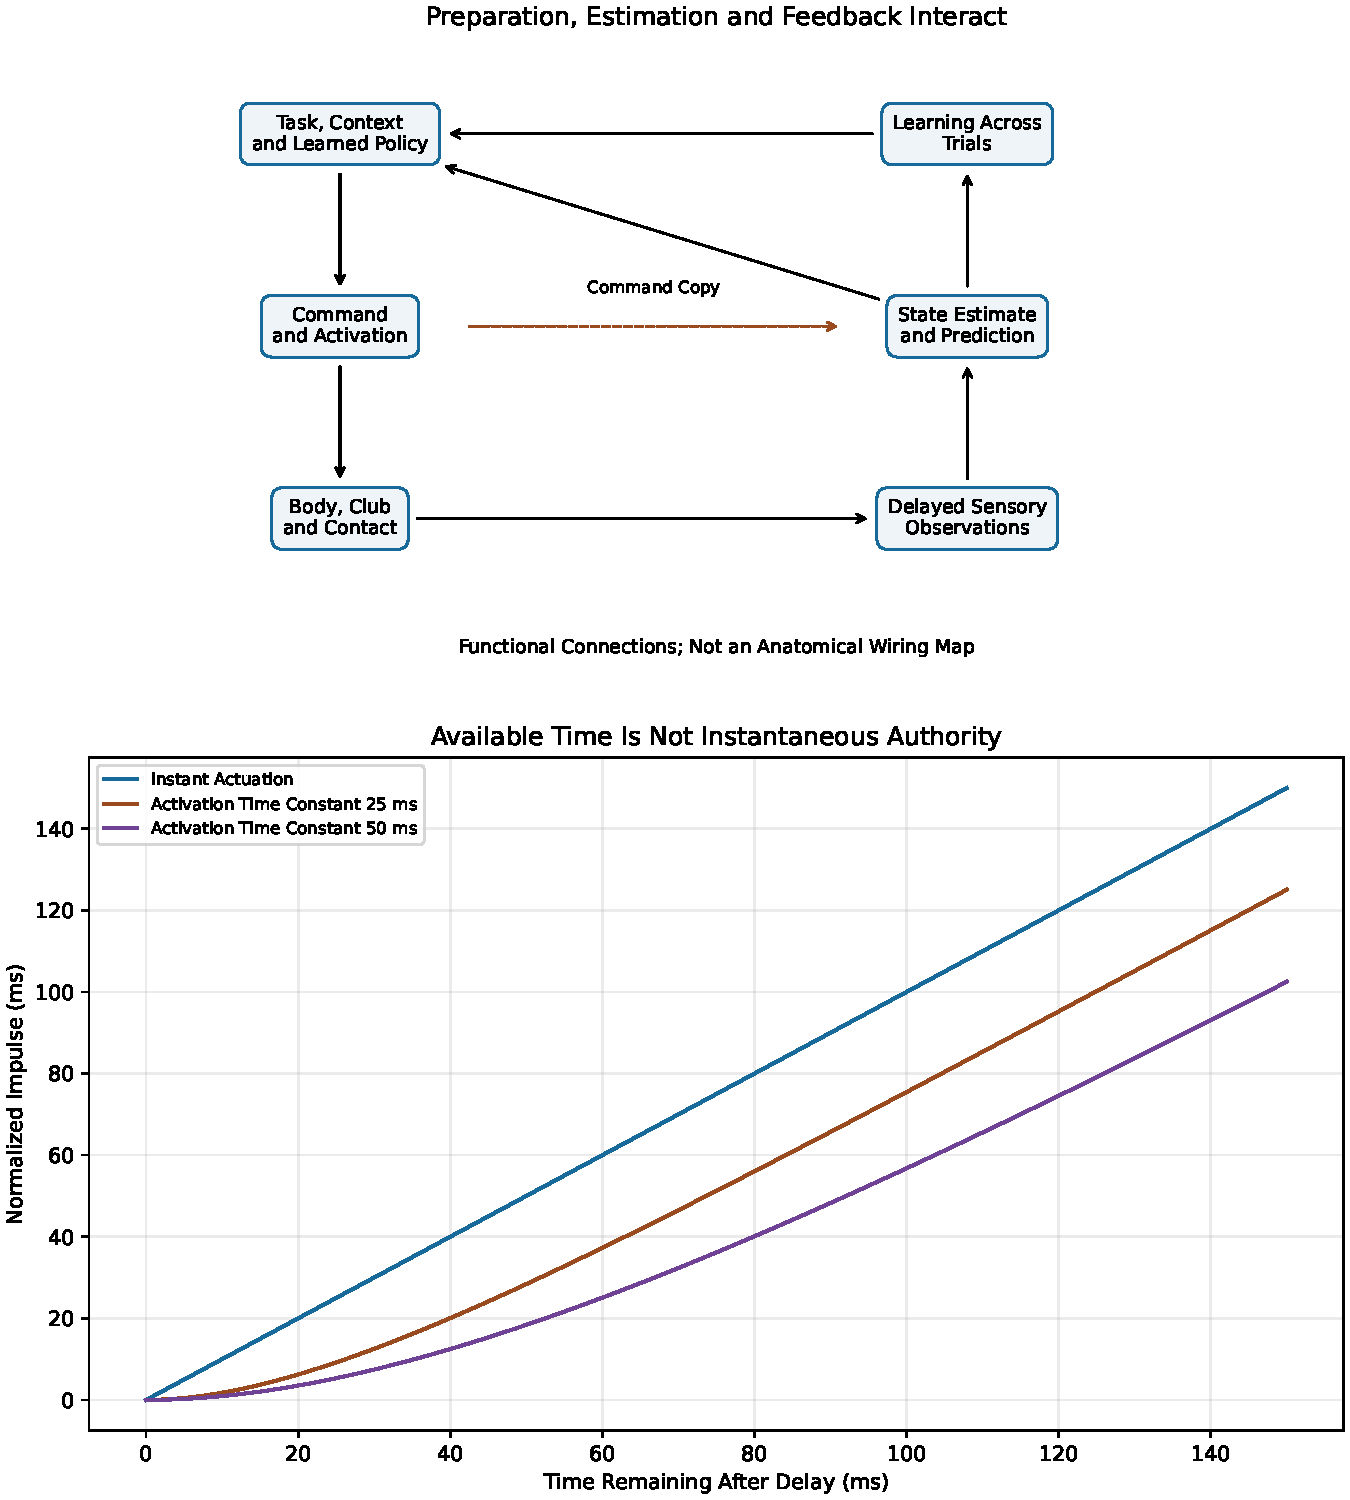
\includegraphics[width=0.9\linewidth,height=0.75\textheight,keepaspectratio]{figures/brain_control_verified.pdf}
\caption{Functional Roles in Control and a Manufactured Activation Example. Preparation, Prediction and Feedback Interact; the Diagram Does Not Assign Each Role to One Brain Region. The Curves Show Normalized Impulse After a Declared Delay, Not Measured Golf Responses.}
\label{fig:ch24_hierarchy}
\end{figure}

\subsection{The Motor Cortex}
\label{subsec:ch24_motor_cortex}
\label{princ:box:ch24_pop_coding}
Motor-cortical activity participates in movement preparation, execution and feedback. A preferred-direction population vector is a useful decoding model under specified conditions, not a complete law that every movement is the vector sum of neuronal votes. Churchland and colleagues reported structured population dynamics during monkey reaching \citep{Churchland2012Dynamics}. This motivates alternatives to a fixed movement-parameter code; it does not establish a unique neural representation for golf or imply that losing neurons has negligible consequences.

\begin{definition}{Descending Pathways and Feedback}{ch24_corticospinal}
The corticospinal tract is one important descending pathway among several. Its origins and connections are more diverse than one M1 neuron controlling one contralateral muscle. Conduction velocity, path length, synapses, recruitment and muscle mechanics all matter when interpreting a response latency. A fastest-fiber speed alone cannot establish the time from an intention to useful joint torque.
\end{definition}

Pruszynski and colleagues used mechanical perturbations in monkeys and stimulation in humans to investigate rapid multijoint feedback. Their findings support an M1 contribution to integrating shoulder and elbow information in responses around 50 ms in those experiments \citep{Pruszynski2011Feedback}. This is evidence that some rapid responses reflect coupled limb mechanics. It does not measure correction of clubface orientation during a golf downswing.

\subsection{The Spinal Cord: Local Regulation Within a Larger Network}
\label{subsec:ch24_spinal_cord}
\begin{definition}{Stretch Responses and Prepared Gain}{ch24_stretch_reflex}
The monosynaptic stretch-reflex pathway includes a muscle-spindle afferent connection to an alpha motor neuron. The observed response also depends on background activation, spinal circuitry and descending modulation. A short response need not await a new conscious decision, but its gain and the state in which it occurs can be prepared beforehand. Calling it wholly independent of the brain loses that distinction.
\end{definition}

\begin{definition}{Central Pattern Generators and Scope}{ch24_cpg}
A central pattern generator is a circuit capable of generating patterned rhythmic output without a matching rhythmic input. Evidence about rhythmic behaviors does not by itself identify a golf-swing CPG. A single prepared swing, a learned feedback policy and a rhythm-generating circuit are different hypotheses.
\end{definition}

Local regulation matters because it acts through the mechanical system. Increasing coactivation may alter impedance before an unexpected perturbation, but also changes force demand, metabolic cost and available torque reserve. Tissue viscosity or stiffness can produce an immediate mechanical response while neural feedback arrives later. Neither guarantees stability: geometry, constraints, damping, delay and active energy supply determine the combined response.

\subsection{The Basal Ganglia, Reward and Credit Assignment}
\label{subsec:ch24_basal_ganglia}
The basal ganglia participate in interacting circuits involved in action and learning; reducing them to an isolated routine selector leaves out that interaction. Dopaminergic activity has been related to reward prediction errors, not simply whether an outcome is objectively good \citep{schultz1997dopamine}.

\begin{definition}{A Motor Program as a Modeling Abstraction}{ch24_motor_program}
A learned action can be represented by a command sequence, a parameterized policy or a combination. Familiarity and automaticity do not establish that brain activity ceases after initiation. Different representations make different predictions when the body or task is perturbed.
\end{definition}

A simple temporal-difference learning model uses
\[
\delta_k=r_k+\gamma V(s_{k+1})-V(s_k),\qquad 0\leq\gamma<1.
\]
Here $r_k$ is reward, $V$ expected future return and $\delta_k$ the reward prediction error. These symbols are not joint angles, muscle energy or sensory discrepancies. Neural reward signals vary by population and task; this model is not a complete dopamine theory.

\begin{example}{Reward Does Not Identify the Effective Part of a Routine}{ch24_bg_golf}
A good shot can follow a poor routine by chance, and a good routine can precede an unlucky outcome. A predicted success need not produce a positive prediction error. Assigning learning to a particular waggle, alignment step or muscle command requires information about what caused the result. Delayed outcomes create a credit-assignment problem; a scalar reward alone does not label the responsible action.

For a terminal outcome with $V(s_{k+1})=0$, expected value 0.8 and reward 1 give $\delta_k=0.2$. Expected value 0.2 with the same reward gives 0.8. The identical result can therefore give different updates in the model. This is not a direct prediction of dopamine firing in a golfer.
\end{example}

Clinical disorders can affect several aspects of movement and learning. They are not controlled deletions of ``action selection'' or ``the internal model,'' and cannot establish universal inability to initiate or perform a particular movement. Mechanistic claims require specific tasks, measurements and appropriate comparison groups.

\subsection{Motor Unit Recruitment and Force Development}
\label{subsec:ch24_recruitment}
\label{princ:box:ch24_size_principle}
A motor unit consists of a motor neuron and the muscle fibers it innervates. Recruitment order and discharge rate both shape the developing force. The size principle describes a tendency for lower-threshold units to be recruited before higher-threshold units under common drive; it is not a serial queue with a compulsory 100--500 ms wait before large units can act. Neural inputs, task and recruitment history matter.

Del Vecchio and colleagues decomposed high-density EMG in tibialis anterior during explosive isometric contractions in 20 men. Recruitment speed and early discharge behavior were associated with rapid force development \citep{DelVecchio2019Recruitment}. Those measurements challenge a universal long recruitment wait. They do not provide recruitment times for every golf muscle, and a motor-unit discharge frequency is not a closed-loop movement bandwidth.

Force development also involves excitation-contraction coupling, contractile behavior, tendon loading and prior activation. Low force does not guarantee precise task control; high force does not prove open-loop control. Signal-dependent variability is a model of how variation changes with drive, not a universal 5--10 percent noise constant. It must specify the measured signal, averaging interval, muscle, task and dependence on force.

\section{Delay, Bandwidth and Time Remaining Before Impact}
\label{sec:ch24_bandwidth}
\label{constr:box:ch24_bandwidth_problem}
Control bandwidth concerns the frequency response of a specified closed loop, with a declared performance criterion. Reaction time is not a neural clock. A flicker-detection threshold is not a motor sampling frequency. Neither the inverse of a response latency nor the frequency of a single shaft mode determines the bandwidth of a coupled golfer-club feedback loop.

\begin{definition}{Delay Adds Phase to a Defined Loop}{ch24_bandwidth}
For a locally linear, time-invariant single-loop approximation,
\[
L(s)=C(s)P(s)e^{-sd},\qquad
\arg e^{-i\omega d}=-\omega d.
\]
The pure delay has unit magnitude and a frequency-dependent phase lag. With $d=0.05$ s, it contributes $-90^\circ$ at 5 Hz and $-180^\circ$ at 10 Hz. Other controller and plant dynamics also contribute phase and gain. These numbers alone do not establish a crossover frequency, stability margin or a maximum human correction rate.
\end{definition}

A shaft frequency also depends on boundary conditions, loading and the mode being measured. The relevant plant includes the body's coupled inertia, contact, actuator dynamics and task output, with properties changing through the swing. For a short nonstationary movement, finite-horizon sensitivity is often more informative than a steady-state bandwidth analogy.

Linearizing an augmented model around a declared nominal motion gives $\delta\dot x=A(t)\delta x+B(t)\delta u$. At a fixed terminal time $T$,
\[
\delta x(T)=\Phi(T,t_0)\delta x(t_0)
+\int_{t_0}^T\Phi(T,s)B(s)\delta u(s)\,ds.
\]
The transition matrix $\Phi$ transports both initial errors and control effects through the changing dynamics. If new information cannot affect $u$ until $t_0+d$, its new-response integral starts there; already prepared commands and other pathways still contribute. Torque limits, activation and output sensitivity determine the attainable change. A norm ratio at one instant does not determine this integral.

\begin{example}{An Actuator Can Begin Responding Without Completing a Correction}{ch24_flicker}
In a manufactured incremental model, let $\dot a=(1-a)/\tau_a$ with $a(0)=0$ after a separately specified pure delay. If the remaining time is $h\geq0$, then
\[
a(h)=1-e^{-h/\tau_a},\qquad
I_a(h)=\int_0^h a(s)\,ds
=h-\tau_a(1-e^{-h/\tau_a}).
\]
$I_a$ has units of time. Multiplication by a constant torque scale gives angular impulse, not directly club-speed change. With $\tau_a=50$ ms, remaining times of 10, 40 and 100 ms give normalized impulses of approximately 0.937, 12.466 and 56.767 ms. Instant actuation would give 10, 40 and 100 ms. Prior activation, state-dependent torque transmission or a different force law changes this comparison.
\end{example}

The impulse example assumes constant mechanical mapping. In the actual linearized chain the kernel $\Phi(T,s)B(s)$ can rotate, amplify or cancel contributions. An EMG onset before impact therefore establishes opportunity for influence, not its sign, size or usefulness.

Impact may also occur at an event time rather than a prescribed clock time. For a smooth event $\psi(x,t)=0$ with transverse nominal crossing,
\[
\delta T=-\frac{\psi_x\,\delta x(T)}{\psi_t+\psi_x F(T)},\qquad
\delta y_{\rm event}=y_x\delta x(T)+(y_t+y_xF(T))\delta T.
\]
$F(T)$ is the nominal state derivative and $\delta x(T)$ the fixed-time perturbation just before the event. These formulas require a nonzero denominator and differentiability; grazing or changing contact modes need separate treatment. A controller can alter arrival time as well as state. Speed at a fixed time and speed at impact are consequently different comparisons.

\section{Variability, Energy and Computation}
\label{sec:ch24_power}
Movement variability does not pass unchanged from a muscle to a club. A local task map with sensitivity $J$ gives $\delta y\simeq J\delta x$, hence
\[
\Sigma_y\simeq J\Sigma_xJ^T.
\]
The covariance includes correlations, not just marginal standard deviations. For two normalized state components with equal standard deviation 0.02 and correlation $\rho$, take $y=(x_1+x_2)/\sqrt2$. Then $\operatorname{var}(y)=0.0004(1+\rho)$. Correlations 0, $-0.75$ and 0.9 give standard deviations 0.0200, 0.0100 and approximately 0.0276. Equal component variability can therefore produce substantially different task variability.

This is a geometric calculation, not evidence that golfers use those correlations. Large sensitivity in one direction can amplify errors while variation in another direction has little immediate effect. Under the same local approximation, the law of total covariance also separates trial-to-trial state uncertainty from conditional observation noise. Measurement error, changing conditions and systematic bias must be accounted for before attributing consistency to a neural strategy.

A coefficient of variation is standard deviation divided by the magnitude of a nonzero mean. A claimed club-speed percentage needs a defined golfer sample, club, instruction, number of trials and instrument uncertainty. It cannot be derived by comparing an unrelated muscle-force percentage with a proprioceptive detection threshold. Drift can amplify or attenuate perturbations depending on the trajectory; its magnitude alone proves neither robustness nor precision.

Mechanical structure influences the controller through these mappings. The same torque can cause different acceleration in different configurations; free acceleration depends on the full inverse inertia, including a Schur-complement effect when other coordinates respond. A constraint changes admissible response, stiffness changes local dynamics, and an actuator's state changes available force. Preparation can alter all of them, while feedback uses information about the resulting state. These mechanisms are intertwined without being interchangeable explanations.

\begin{principle}{Separate Mechanical Work, Metabolic Cost and Computation}{box:ch24_power_budget}
Joint mechanical power is torque times joint rate; net negative work, positive work and coactivation have different physiological implications. A controller's metabolic expenditure is a different quantity. An estimate of whole-brain power cannot be assigned entirely to swing computation or converted into a known number of optimization iterations.

Counting neurons, synapses or spikes does not identify the arithmetic operations needed by a digital optimizer. Even a specified state dimension does not determine solve time: horizon, discretization, constraints, sparsity, numerical conditioning, solver, hardware and accuracy all matter. A valid efficiency comparison specifies the task, performance, energy boundary and measurement protocol.
\end{principle}

\begin{example}{Online Control and Learning Across Trials}{ch24_online_vs_offline}
A robot with a 1 ms command period needs sensing, estimation, computation and command transmission to meet that deadline, or an explicitly designed asynchronous policy. A 20-state description alone does not show whether this is feasible. A learned policy can be quick to evaluate and still depend on feedback; an optimizer can also be warm-started from previous solutions. Neither architecture follows from the word ``robot.''

Likewise, practice can alter prepared commands, prediction, sensory weighting and feedback gains. The relevant test is what changes in behavior and response to perturbations, including retention and transfer, rather than whether the action appears effortless.
\end{example}

\begin{principle}{Key Takeaways}{box:ch24_takeaways}
The mechanical model defines what force can do; the observation model defines what can be inferred; the actuator model and time remaining define which changes are feasible. A policy connects them to a task, and learning changes the policy or model over experience. No one instantaneous ratio, neural delay or brain region replaces this chain of reasoning.

Golf-specific perturbation evidence is needed to quantify the relative contributions of parallel pathways during a downswing. A useful study measures perturbation time, muscle response, force or torque, body and club motion, event time and strike outcome. Similar motions can be produced by different controllers, so a successful fit is not automatically identification of the neural mechanism.
\end{principle}



\begin{exercises}{Chapter Exercises and Worked Answers}{ex:ch24_exercises}
\subsection*{1. Correct the Forward Prediction}
A model outputs $\dot x=(2,-4)^T$ in the appropriate state units per second, with current state $x=(1,3)^T$ and step $\Delta t=0.01$ s. Compute one Euler step and explain its limit.

\textbf{Worked answer.} The prediction is $(1.02,2.96)^T$. It adds a change to the existing state. Equating the next state directly to $(2,-4)^T$ is dimensionally wrong. Smoothness gives local error of order $\Delta t^2$; this estimate alone does not verify the model or numerical stability over a whole swing.

\subsection*{2. Diagnose an Infeasible Inverse}
For the normalized rectangular example above, compute the bounded input and residual. Does failure of instantaneous position control prove that positions can never be controlled?

\textbf{Worked answer.} Minimizing $1+(u-3)^2+u^2$ gives unconstrained $u=1.5$, or bounded $u=1$ with $|u|\leq1$. The desired-minus-achieved residual is $(0,1,2,-1)^T$. It exposes both the kinematic mismatch and conflicting acceleration requests. Over time, acceleration affects position; finite-time reachability must be analyzed through the dynamics, not from the zero position block alone.

\subsection*{3. Compare Delay With Activation}
A new response has a separately defined delay of 50 ms. Impact is 90 ms after the perturbation. In the chapter's zero-initial-state actuator with $\tau_a=50$ ms, what time remains, and what is its normalized impulse?

\textbf{Worked answer.} The remaining time is 40 ms. The normalized impulse is $0.04-0.05(1-e^{-0.8})\simeq0.012466$ s. Multiplying by a constant 10 N m scale gives approximately 0.12466 N m s. Computing a club velocity additionally requires the mechanical response map. The example does not erase pre-existing activation or responses in other pathways.

\subsection*{4. Interpret a Frequency Comparison}
A pure delay is 50 ms. Calculate its phase at 5 Hz and explain why a shaft mode at that frequency does not determine whether the full loop is stable.

\textbf{Worked answer.} The lag is $-2\pi(5)(0.05)=-\pi/2$ radians, or $-90^\circ$. Stability depends on the full open-loop gain and phase, including the plant and controller, and on the chosen approximation. A shaft mode under one support condition is neither the whole plant nor a sampling rate. Nonstationary strike tasks also need finite-time analysis.

\subsection*{5. Explain Consistency Without Inventing a Noise Constant}
Use the two-component covariance example. What happens when the correlation changes from 0 to $-0.75$, and what would be needed to apply the result to golf?

\textbf{Worked answer.} Task variance falls from 0.0004 to 0.0001 and its standard deviation halves. The marginal component deviations remain 0.02. A golf application requires a measured covariance in declared coordinates, a validated task sensitivity and instrument uncertainty. It also needs event-time effects if trials are compared at impact. The example cannot establish a universal club-speed coefficient of variation or an automatic stabilizing role for drift.

\subsection*{6. Distinguish Three Errors}
A player correctly predicts that a shot will miss the target. The outcome is nevertheless better than expected in the scoring system. Identify the sensory prediction, task and reward errors.

\textbf{Worked answer.} The observed consequence can have a small sensory prediction error, a substantial task error and a positive reward prediction error. Their dimensions and reference values differ. One scalar reward does not specify which muscle, state estimate or pre-shot action should change.

\subsection*{7. Test the Free-Energy Identity}
For joint probabilities $p(y,z)=(0.12,0.18)$, compute the evidence and the minimizing belief. Does minimizing variational free energy demonstrate a reduction in mechanical energy?

\textbf{Worked answer.} The evidence is 0.30 and the posterior belief is $(0.4,0.6)$. At that belief the KL term vanishes and $\mathcal F=-\log0.30\simeq1.204$ with natural logarithms. A different belief adds a nonnegative KL term. This is an information-theoretic identity, not a mechanical or metabolic energy budget and not proof of a neural implementation.

\subsection*{8. Evaluate a Recruitment Claim}
Does size-ordered recruitment require waiting a fixed interval before higher-threshold units contribute? What measurements distinguish recruitment from force development?

\textbf{Worked answer.} Recruitment order does not prescribe a universal serial waiting time. Recruitment speed, discharge behavior, prior activation and contractile transmission jointly affect force. Measure motor-unit or appropriately interpreted EMG activity and force with synchronized timing. Evidence from an explosive isometric leg task cannot simply be assigned to a wrist during a swing.

\subsection*{9. Design a Controller Comparison}
Compare a prepared command sequence with a learned feedback policy. What information is missing from a proposal to solve a 20-state optimization every millisecond?

\textbf{Worked answer.} Perturb the movement in a controlled way and compare subsequent commands and task outcomes, accounting for delays and actuator state. Similar unperturbed trajectories need not reveal which architecture generated them. For computation, specify horizon, objective, constraints, discretization, solver tolerance, hardware and sensing/transmission time. State dimension and movement duration alone cannot yield a minimum computation time.

\subsection*{10. What Would Establish Useful Within-Swing Correction?}
Design a golf experiment that separates response onset from useful response authority, while allowing learning between trials.

\textbf{Worked answer.} Apply safe, controlled perturbations at declared phases with randomized timing and appropriate comparison trials. Record synchronized muscle activity, mechanical response, club pose and velocity, impact time and strike outcome. Estimate uncertainty and distinguish local changes from improvements in the task. Compare early and late perturbations, repeated exposure and retention; control equipment, instruction and starting state. An early EMG difference shows a response, while a reliable task improvement requires mechanical and outcome evidence. Attribution to a particular neural pathway requires additional evidence beyond timing alone.
\end{exercises}
\flushbottom{}
\newpage
